\documentclass[oneside,reqno]{amsart}
\usepackage{amsthm}
\usepackage{dsfont}
\setlength{\textwidth}{\paperwidth}\addtolength{\textwidth}{-2in}\calclayout
\usepackage[utf8]{inputenc}
\usepackage{tikz}
\usepackage{minted}
\newminted{python3}{frame=lines}
\usepackage{booktabs}
\usepackage{enumitem}

\DeclareMathOperator{\E}{E}
\DeclareMathOperator{\var}{var}
\DeclareMathOperator{\cov}{cov}
\DeclareMathOperator{\corr}{corr}
\DeclareMathOperator{\tr}{tr}
\let\vec\relax\DeclareMathOperator{\vec}{vec}
\newcommand{\eps}{\varepsilon}
\newcommand{\ups}{\upsilon}
\newcommand{\M}{\mathcal{M}}
\newcommand{\N}{\mathrm N}

\theoremstyle{definition}
\newtheorem{prob}{Problem}
\renewcommand*{\proofname}{Solution}
\setlist[enumerate]{label={(\roman*)}}


\title{ECON 706: Problem Set 6}
\author{Daniel Pfeffer}
\date{\today}
%------------------------------------------------------------------------------
\begin{document}
\maketitle

\begin{prob}
Consider the class of AR($p$) models with intercept: 
\begin{equation}\label{eq:arp}
	y_t =  c +\phi_1 y_{t-1} + \cdots + \phi_p y_{t-p} + \eps_t, 
	\qquad 
	\eps_t \sim \N(0, \sigma^2)
\end{equation}
with prior distribution 
\begin{equation}\label{eq:arp-prior}
	\phi \mid \sigma^2 \sim \N(\phi_0, \sigma^2 V_0),
	\qquad 
	p(\sigma^2) \propto \frac{1}{\sigma^2}. 
\end{equation}
\end{prob}

\begin{enumerate}
\item
What is $\log p(y \mid \sigma^2)$? 

\begin{proof}
Let $X = (1,y_{t-1},\dotsc,y_{t-p})'$ and $\phi = (c, \phi_1,\dotsc,\phi_p)'$, and let $y = (y_1, y_2,\dotsc,y_T)'$ be a $T \times 1$ vector of observations. Then combining likelihood with the prior gives the conditional posterior:
\begin{align*}
	p(\phi \mid y, \sigma^2) &\propto p(y \mid \phi, \sigma^2) p(\phi \mid \sigma^2) \\
	& \propto \exp\left( -\frac{1}{2\sigma^2}(y - X \phi)' (y - X \phi) \right)
	\exp\left(-\frac{1}{2 \sigma^2} (\phi - \phi_0)'  V_0^{-1} (\phi - \phi_0)\right) \\
	&\propto\exp\left(-\frac{1}{2 \sigma^2} ( \phi' V_0^{-1}\phi - 2 \phi' X'y - \phi' X'X \phi - 2 \phi' V_0 \phi_0)\right) \\
	&\propto \exp\left(-\frac{1}{2 \sigma^2} (\phi'(X'X + V_0^{-1}) \phi - 2 \phi'( X'y+ V_0^{-1} \phi_0)+ \phi_0' V_0^{-1} \phi_0 )\right).
\end{align*}
If we define 
\begin{align*}
	\phi_1 &= (X'X + V_0^{-1})^{-1}(X'y +  V_0^{-1} \phi_0) \\
	V_1 &= (X'X + V_0^{-1})^{-1},
\end{align*}
then,
\begin{align*}
	p(\phi \mid y, \sigma^2) &\propto \exp\left(-\frac{1}{2 \sigma^2} \left((\phi - \phi_1)'V_1^{-1}(\phi-\phi_1) + \phi_0'V_0^{-1}\phi_0 - \phi_1V_1^{-1}\phi_1 \right)\right) \\
	&\propto \exp\left(-\frac{1}{2 \sigma^2} (\phi - \phi_1)'V_1^{-1}(\phi-\phi_1)\right).
\end{align*}
Hence the posterior is Gaussian:
\[
	\phi \mid (y, \sigma^2) \sim \N(\phi_1, V_1)
\]
\par
To derive the marginal likelihood, note that
\begin{align*}
	p(\phi\mid \sigma^2)  &\overset{d}{=} \N(\phi_0, \sigma^2  V_0) \\
	p(\phi\mid y, \sigma^2) &\overset{d}{=} \N(\phi_1, \sigma^2  V_1),
\end{align*}
and ``invert'' Bayes' theorem to obtain
\begin{align*}
	 p(y \mid \sigma^2)  & = \frac{p(y \mid \phi, \sigma^2) p(\phi \mid \sigma^2)}{p(\phi \mid y, \sigma^2)}\\
	&= \frac{(2\pi \sigma^2)^{-T/2} \exp((2 \sigma^2)^{-1} y'y) (2\pi)^{-k/2}  |\sigma^2  V_0 |^{-1/2}  \exp((2 \sigma^2)^{-1}  \phi_0'   V_0^{-1} \phi_0)}{ (2\pi)^{-k/2} |\sigma^2  V_1 |^{-1/2} \exp((2 \sigma^2)^{-1} \phi_1'   V_1^{-1}  \phi_1)} \\
	&= (2\pi \sigma^2)^{-T/2} \frac{| V_0 |^{-1/2}}{| V_1|^{-1/2}}\exp\left(- \frac{1}{2 \sigma^2} \left(y'y + \phi_0'  V_0^{-1} \phi_0 -    \phi_1'  V_1^{-1}  \phi_1 \right) \right),
\end{align*}	
which follows from the fact that the $\phi$ terms must cancel. The log marginal likelihood is then 
\[
	\log p(y \mid \sigma^2) 
	= -\frac{T}{2} \log (2\pi \sigma^2) - \frac{1}{2}\log\frac{| V_0|}{| V_1|} -\frac{1}{2 \sigma^2} \left(y'y+  \phi_0'  V_0^{-1}  \phi_0 -  \phi_1'  V_1^{-1}  \phi_1 \right).
\]
\end{proof}

\item
Collect data on real GDP growth from FRED for the period from 1984:Q1 to 2015:Q4. Figure \ref{gdp-growth} plots the data.

\begin{python3code}
import numpy as np
import matplotlib.pyplot as plt
import pandas_datareader.data as web
import datetime

# Query data
start = datetime.datetime(1984, 10, 1)
end = datetime.datetime(2015, 12, 31)
ts = web.DataReader('GDPC1', 'fred', start, end)
ts = 4*np.log(ts).diff().dropna()

# Plot data
plt.figure(figsize=(9,6))
plt.plot(ts)
plt.ylabel('GDP Growth')
plt.title('Annualized Quarter-on-Quarter GDP Growth Rates')
plt.show()
\end{python3code}

\begin{figure}
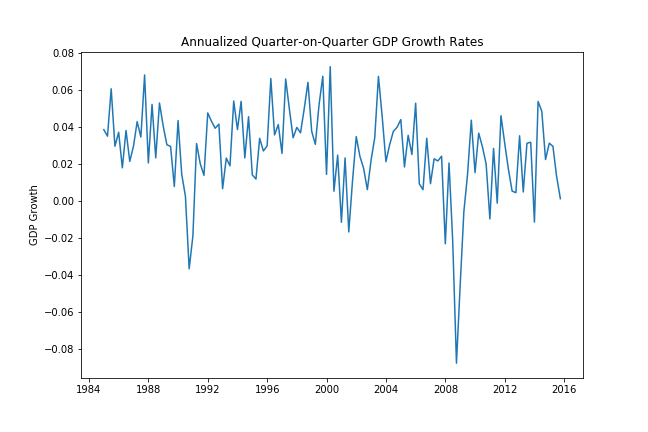
\includegraphics[width=\textwidth]{gdp-growth}
\caption{}
\label{gdp-growth}
\end{figure}

\item
The goal is to determine the ``correct" number of lags for the AR model. We will regard each lag length $p$ as a separate model $\M_p$. The computation of posterior probabilities requires $\log p(y \mid \M_p)$. To simplify the calculations a bit, we use $\log p(y \mid \hat \sigma^2, \M_p)$ instead, where 
\[
	\hat \sigma^2 = (y - X \phi_1)' (y-X\phi_1)/T.
\]
Here $\phi_1$ is the posterior mean. Choose numerical values for $\phi_0$, and $V_0$ for models $\M_1$ to $\M_4$ and compute $\log p(y \mid \hat \sigma^2, \M_p)$ for $y$ ranging form 1985:Q1 to 2015:Q4. (Note that you need the 1984 observations to initialize lags).

\begin{proof}
Fit the model.
\begin{python3code}
def ar_bayes(df, lags, tau): 
    y = df['GDPC1'][lags:]
    X = df
    # Model i data
    for col in X.columns:
        for l in range(1,lags+1):
            X.loc[:,col+"_L"+str(l)] = X[col].shift(l)
    X = df.drop(['GDPC1'], axis=1).dropna()
    from statsmodels.api import add_constant
    X = add_constant(X)
    T = len(ts) - lags
    
    from numpy.linalg import inv, det
    # Prior means and covariance matrices
    phi_0 = np.zeros(lags+1)
    V_0 = tau*np.eye(lags+1)
    
    # Posterior means and covariance matrices
    V_1 = inv(X.T @ X + inv(V_0))
    phi_1 = V_1 @ (X.T @ y + inv(V_0) @ phi_0.T)
    
    sigma2 = ((y - X @ phi_1).T @ (y - X @ phi_1))/T
    
    mdd = -T/2*np.log(2*np.pi*sigma2) \
                      - 0.5*np.log(det(V_0)/det(V_1)) \
            - 0.5/sigma2*(y.T @ y + phi_0.T @ inv(V_0) \
               @ phi_0 - phi_1.T @ inv(V_1) @ phi_1) 

    return {'phi_1':phi_1, 'V_1': V_1, 'mdd':mdd} 

# Marginal likelihoods
mdds = []
for i in range(1, 5):
    mdds.append(ar_bayes(ts[:], i, tau=10)['mdd'])
mdds
\end{python3code}

The marginal data density values are $285.03$, $284.28$, $ 282.36$, and $279.41$ for models $\M_1$, $\M_2$, $\M_3$, and $\M_4$, respectively. The optimal lag order is therefore one.
\end{proof}

\item
Convert the $\log p(y \mid \hat \sigma^2, \M_p)$ into posterior model probabilities (you need to assume some prior model probabilities). If you had to select a lag order, which one would you select? If you would average predictions across models, which of the model specifications would receive non-trivial weight?


\begin{proof}
The following computes the posterior model probabilities, where the prior is such that the prior probability or each lag order is equal.
\begin{python3code}
# Log posterior probabilities
mod_prior = [0.25, 0.25, 0.25, 0.25]
denom = 0.25*np.sum(np.exp(mdds))
mod_post_prob = []
for i in range(4):
    mod_post_prob.append(0.25*np.exp(mdds[i])/denom)
mod_post_prob
\end{python3code}

The posterior model probabilities are $0.65$, $0.31$, $0.05$, and $0.002$, for models $\M_1$, $\M_2$, $\M_3$, and $\M_4$, respectively. 
\end{proof}

\item
Now suppose that you condition on the model with the preferred lag
order $\hat p$. Suppose that you introduce a hyperparameter $\tau$ and change your prior to
\begin{equation}
	\phi \mid \sigma^2 \sim \N(\phi_0, \sigma^2\tau V_0).
\end{equation}
Now compute $p(y \mid \tau, \hat \sigma^2, \M_{\hat p})$ for values of $\tau$ on the grid 
\[
	\frac{1}{100}, \frac{1}{10}, 1, 10, 100.
\]
Which scaling of the prior covariance matrix is preferred?

\begin{proof}
The following code computes the marginal data density (conditional on $\tau$).
\begin{python3code}
# Generate grid
hyper_mdds = []
taus = [1/1000] * 6
for i in range(1,5):
    taus[i+1] = taus[i]*10
    hyper_mdds.append(ar_bayes(ts[:], lags=1, tau=taus[i])['mdd'])
hyper_mdds
\end{python3code}

The marginal likelihoods conditional on $\tau$ are $240.35$, $256.88$, $278.64$, and $282.93$. So the preferred scaling is where $\tau=0.01$.
\end{proof}
\end{enumerate}

\subsection*{Problem 2}
Consider the state-space model:
\begin{align}\label{eq:state-space}
\begin{split}
	y_t = \lambda s_t + \ups_t   \\
	s_t = \phi s_{t-1} + \eps_t.
\end{split}
\end{align}
For now assume that $\ups_t \sim \text{iid }\N(0,1)$, $\eps_t \sim \text{iid }\N(0,1)$, and $\ups_t \perp\eps_t$.
\begin{enumerate}
\item
Derive the autocovariance function for $y_t$.

\begin{proof}
Since state equation is an AR(1) process, its autocovariance function is
\begin{align*}
	\gamma_s(h)  = \begin{cases}
		1/(1-\phi^2) & \text{if } h = 0 \\
		\phi^{|h|}/(1-\phi^2) & \text{if } h \neq 0.				
	\end{cases}
\end{align*}
Since $\ups_t$ and $\eps_t$ are orthogonal at all leads and lags, 
\begin{align*}
	\gamma_y(0) &= \var(y_t) = \var(\lambda s_t + \ups_t) 
		= \gamma_s(0)\lambda^2 + 1 
		= \frac{\lambda^2}{1-\phi^2} + 1 \\
	\gamma_y(h) &= \cov(\lambda s_t + \ups_t, \lambda s_{t-h} + \ups_{t-h}) 
		= \gamma_s(0) \lambda^2 \phi^{|h|} = \frac{\lambda^2}{1-\phi^2} \phi^{|h|}, \qquad h \neq 0.
\end{align*}
\end{proof}

\item
Are the coefficients of the state-space model identified?

\begin{proof}
No. The factor loading $\lambda$ is unique only up an orthogonal transformation and therefore is not sign-identified. To see this point, let $\tilde s_t = -s_t$ and let $\tilde\eps_t = -\eps_t$, and 
\[
	y_t = -\lambda \tilde s_t + \ups_t, \qquad \tilde s_t = \phi \tilde s_{t-1} + \tilde\eps_t.
\]
Then 
\begin{align*}
	y_t &= -\lambda (\phi \tilde s_{t-1} + \tilde\eps_t) + \ups_t \\
	&= -\lambda (\phi (- s_{t-1}) + (-\eps_t)) + \ups_t \\
	&= \lambda (\phi s_{t-1}  + \eps_t) + \ups_t,
\end{align*}
which is observationally equivalent to the state-space representation \eqref{eq:state-space} since it has the same autocorrelation function.
\end{proof}

\item
Find an observationally equivalent ARMA representation for the state-space model. Express the ARMA parameters as functions of $(\lambda, \phi)$. 

\begin{proof}
Subtract $\phi y_{t-1}$ from both sides of the observation equation to obtain 
\[
	y_t - \phi y_{t-1} = \lambda s_t + \ups_t - \lambda \phi s_{t-1} - \phi \ups_{t-1} 
\]	
or 
\[
	y_t = \phi y_{t-1} + \lambda \eps_t + \ups_t + \phi \ups_{t-1}.
\]
This resembles an ARMA(1,1) process:
\[
	y_t = \rho y_{t-1} + \eta_t + \theta \eta_{t-1}, 
	\qquad \eta_t  \sim \text{iid } \N(0, \sigma_\eta^2),
\]
which has covariance structure 
\begin{align*}
	\gamma_y(0) &= \sigma_\eta^2 \frac{1+\theta^2 + 2 \theta \rho}{1-\rho^2}  \\
	\gamma_y(1) &= \sigma_\eta^2\frac{(1+  \theta \rho)(\rho +\theta)}{1-\rho^2}\\
	\gamma_y(h) &= \gamma_y(1)  \rho^{|h|-1}, \qquad |h| \geq 1.
\end{align*}
To obtain an observationally equivalent ARMA representation, we will match autocovariance functions. Evidently, for $h>1$, we require $\rho = \phi$, which gives the following $2 \times 2$ system:
\begin{align*}
	\gamma_y(0)(1-\phi^2) &= (1+\theta^2 + 2 \theta \phi) \sigma_\eta^2  = 1-\phi^2 + \lambda^2 \\
	\gamma_y(1)(1-\phi^2) &= (\theta - \theta \phi + 1 + \theta^2 + 2 \theta \phi) \sigma_\eta^2  = \phi.
\end{align*}
Subtracting the corresponding equations gives 
\begin{align*}
	\gamma_y(0)(1-\phi^2) &= (1+\theta^2 + 2 \theta \phi) \sigma_\eta^2  = 1-\phi^2+ \lambda \\
	\gamma_y(1)(1-\phi^2) &= (\theta - \theta \phi + 1 + \theta^2 + 2 \theta \phi) \sigma_\eta^2  = \phi \lambda^2,
\end{align*}
and divide the second equation here by $\phi$ and subtracted it from the first equation to obtain 
\begin{align*}
	\sigma_\eta^2\theta(1-\phi^2)/\phi &= - (1-\phi^2) \\
	\sigma_\eta^2 = -\phi/\theta.
\end{align*}
Now substitute this into the first equation:
\begin{align*}
	-\phi(1 + 2 \theta\phi + \theta^2 )/ \theta &= 1 - \phi^2 + \lambda^2 \\
	-\phi(1 + 2 \theta\phi + \theta^2 ) &= \theta - \theta \phi^2 + \theta \lambda^2
\end{align*}
or 
\[
	\phi \theta^2 + \theta(\phi^2 + \lambda^2 + 1) + \phi = 0
\]
This quadratic equation in $\theta$ has two solutions given by
\[
	\theta = \frac{-(\phi^2 + \lambda^2 + 1) \pm \sqrt{(\phi^2 + \lambda^2 + 1)^2 - 4 \phi^2}}{2 \phi}
\]
To obtain a single solution, we can require that the ARMA(1,1) process is invertible (i.e., $|\theta| < 1$): 
\begin{align*}
	\theta &= \frac{-(\phi^2 + \lambda^2 + 1) + \sqrt{(\phi^2 + \lambda^2 + 1)^2 - 4 \phi^2}}{2 \phi} \\
	\sigma_\eta^2 &= -\frac{\phi}{\theta} = \frac{2}{(\phi^2 + \lambda^2 + 1) - \sqrt{(\phi^2 + \lambda^2 + 1) - 4 \phi^2}}.
\end{align*}
\end{proof}


\item
Now suppose that $\ups_t$ and $\eps_t$ are jointly normally distributed and have a correlation $\rho$. Re-derive the autocovariance function for $y_t$. Are the coefficients $(\lambda, \phi, \rho)$ identified? Find an observationally equivalent ARMA representation.

\begin{proof}
To find autocovariance function for $y_t$ when there is a non-zero correlation $\rho$ between $\ups_t$ and $\eps_t$, we simply add the cross product to our earlier calculations and obtain 
\begin{align*}
	\gamma_y(0) &= \frac{\lambda^2}{1-\phi^2} + 2 \lambda \rho \\
	\gamma_y(h) &=  \left(\frac{\lambda^2}{1-\rho^2} + \lambda \rho \right)\phi^{|h|} , \qquad h \neq 0,
\end{align*}
which imply that although $\lambda \rho$ is sign-identified, neither $\lambda$ nor $\phi$ nor $\rho$ is uniquely identified. 
\par
Write the observationally equivalent ARMA(1,1) process as
\[
	y_t = \rho y_{t-1} -\eta_1 + \theta \eta_{t-1},
	\qquad \eta_t \sim \text{iid } \N(0, \eta_t^2).
\]
Matching autocovariance functions as in (iii) gives
\[
	\sigma_\eta^2 = - \phi(1 + \lambda \rho)/\theta,
\]
with solution 
\begin{align*}
	\theta &= \frac{-(\phi^2 + \lambda^2 + 1 + 2 \lambda \rho) + \sqrt{(\phi^2 + \lambda^2 + 1 + 2 \lambda \rho)^2 - 4 \phi^2 (1 + \lambda \rho)^2}}{2 \phi (1 + \lambda \rho)} \\
	\sigma_\eta^2 &= -\frac{\phi}{\theta} = \frac{2 (1 + \lambda \rho)}{(\phi^2 + \lambda^2 + 1 + 2 \lambda \rho) - \sqrt{(\phi^2 + \lambda^2 + 1 + 2 \lambda \rho)^2 - 4 \phi^2 (1 + \lambda \rho)^2}}.
\end{align*}
\end{proof}

\item
We derived the Kalman filter iterations under the assumption that the errors in the measurement equation and the state-transition equation are independent. Generalize the Kalman filter iterations for the above state-space model to allow for a non-zero correlation $\rho$ between $\ups_t$ and $\eps_t$. 

\begin{proof}
Initialize the recursion by assuming that state vector has the unconditional distribution distribution $s_0 \sim \N(\bar s_0, p_0)$, with 
\begin{align*}
	\bar s_0 &= \E s_0 = 0 \\
	p_0 &= \var(s_0) = \frac{1}{1-\phi^2}. 
\end{align*}
Assume that at time $t$ the previous iteration yields 
\[	
	s_{t-1} \mid y^{t-1} \sim \N(\bar s_{t-1|t-1}, p_{t-1|t-1}).
\]
\begin{enumerate}[label=(\arabic*)]
\item
Forecast: Our assumptions together with $\eps_t \sim \text{iid } \N(0,1)$ imply that 
\[
	s_t \mid y^{t-1} \sim \N(\bar s_{t\mid t-1}, p_{t\mid t-1}),
\] 
where 
\begin{align*}
	\bar s_{t+1 \mid t} &= \E(s_t \mid y^{t-1}) 
		= \phi \bar s_{t-1\mid t-1} \\
	 p_{t \mid t-1} &= \var(s_t \mid y^{t-1}) 
	 	= \phi^2  p_{t-1 \mid t-1}  + 1.
\end{align*}
\item
Likelihood: The marginal distribution of $y_t$ conditional on $y^{t-1}$ is of the form 
\[
	y_t \mid y^{t-1} \sim \N(\bar y_{t \mid t-1}, f_{t\mid t-1}),
\] 
where 
\begin{align*}
	\bar y_{t \mid t-1} &= \E(y_t \mid y^{t-1})
		 = \lambda \bar s_{t \mid t-1} \\
	 f_{t \mid t-1} &= \var(y_t \mid y^{t-1}) 
	 	= \lambda^2 p_{t \mid t-1} +1 + 2 \lambda^2 \rho.
\end{align*}
\item
Update: The joint distribution of the $s_t$ and $y_t$ is 
\[
	\begin{pmatrix}
		s_t \\ y_t 
	\end{pmatrix}
	\mid y^{t-1} \sim \N
	\begin{pmatrix}
		\begin{pmatrix}
			\bar s_{t\mid t-1}  \\ 
			\bar y_{t \mid t-1} 
		\end{pmatrix},
		\begin{pmatrix}
			p_{t \mid t-1} & \lambda p_{t \mid t-1} + \rho \\
			\lambda p_{t \mid t-1} + \rho & f_{t \mid t-1}
		\end{pmatrix}
	\end{pmatrix},
\]
where the covariance captures the correlation between $\ups_t$ and $\eps_t$ and is obtained from
\begin{align*}
	\cov(s_t, y_t \mid y^{t-1}) &= \cov(s_t, \lambda s_t + \ups_t \mid y^{t-1}) \\
	&= \lambda \var(s_t\mid y^{t-1}) + \cov(\phi s_{t-1} + \eps_t, \ups_t\mid y^{t-1}) \\
	&= \lambda p_{t \mid t-1} + \rho 
\end{align*}
Applying Bayes' Theorem gives 
\[
	s_t \mid (y_t, y^{t-1}) \sim \N(\bar s_{t\mid t}, p_{t\mid t}),
\]
where 
\begin{align*}
	\bar s_{t\mid t} &= \bar s_{t\mid t-1} + (\lambda p_{t \mid t-1} + \rho) (y_t - \bar y_{t\mid t-1})/ f_{t \mid t-1} \\
	p_{t \mid t} &= p_{t \mid t-1} -  (\lambda p_{t \mid t-1} + \rho)^2 / f_{t \mid t-1}
\end{align*}
\end{enumerate}
This completes one iteration of the Kalman filter.
\end{proof}

\end{enumerate}


\end{document}

\begin{align*}
	p(\phi \mid y, \sigma^2) &\propto p(y \mid \phi, \sigma^2) p(\phi \mid \sigma^2) \\
	& \propto \exp\left( -\frac{1}{2\sigma^2}(y- X \phi)' (y-X \phi) \right)
	\exp\left( - \frac{1}{2 \sigma^2} (\phi - \phi_0)'  V_0^{-1} (\phi - \phi_0)\right) \\
	&\propto\exp\left(-\frac{1}{2 \sigma^2} \left(y'y- 2 \phi' X'y- \phi'X'X\phi + \phi' V_0^{-1}\phi - 2 \phi' V_0 \phi_0 + \phi_0' V_0^{-1}  \phi_0 \right)\right) \\
	&\propto \exp\left(-\frac{1}{2 \sigma^2} \left(y'y- 2 \phi'( X'y+ V_0^{-1} \phi_0) + \phi'(X'X + V_0^{-1}) \phi + \phi_0' V_0^{-1} \phi_0 \right)\right).
\end{align*}

